% CE520 Graduate Seminar flyer — Bilge Evran, Fall 2026
% Compile with pdfLaTeX (Overleaf compatible).
% Keep metu-logo.png in the same directory as this .tex file.
\documentclass[10pt,a4paper]{article}
\usepackage[margin=13mm,top=11mm,bottom=12mm]{geometry}
\usepackage[T1]{fontenc}
\usepackage[utf8]{inputenc}
\usepackage{lmodern}
\usepackage[scaled=0.95]{helvet}
\renewcommand{\familydefault}{\sfdefault}
\usepackage{graphicx,tabularx,array,microtype}
\usepackage{tikz}
\usetikzlibrary{arrows.meta,positioning,calc,shapes.geometric}
\usepackage[most]{tcolorbox}
\usepackage{xcolor}
\usepackage{enumitem}
\usepackage{hyperref}
\hypersetup{hidelinks}
\pagestyle{empty}
\setlength{\parindent}{0pt}
\setlength{\parskip}{0pt}
\setlength{\fboxsep}{0pt}

% ---- Editable seminar details ----
\newcommand{\SpeakerName}{Bilge Kutay}
\newcommand{\SupervisorName}{Asst. Prof. Dr. Cüneyt Baykal}
\newcommand{\SeminarDate}{November 11 2026}
\newcommand{\SeminarTime}{13.40-13.55}
\newcommand{\SeminarRoom}{METU Civil Engineering Depatment K1 Building (Room CES23)}
\newcommand{\SpeakerEmail}{bilge.kutay@metu.edu.tr}
% You can change the title or subtitle here.
\newcommand{\ThesisTalkTitle}{Machine-Learning-Based Active Wave Absorption\\in a Numerical Wave Flume}
\newcommand{\ThesisTalkSubtitle}{Numerical modelling and piston-type wavemaker control using OpenFOAM}

\definecolor{metured}{HTML}{AE0F16}
\definecolor{deepred}{HTML}{8B1016}
\definecolor{ink}{HTML}{1D2832}
\definecolor{muted}{HTML}{5C6670}
\definecolor{cloud}{HTML}{F3F4F6}
\definecolor{teal}{HTML}{087C8C}
\definecolor{waveblue}{HTML}{0675AC}
\definecolor{lightwater}{HTML}{DDF1F9}
\definecolor{navy}{HTML}{23475E}
\color{ink}


\newcommand{\SectionHeading}[1]{%
  \par\vspace{3mm}\noindent{\color{metured}\bfseries\fontsize{12}{13}\selectfont #1}\par
  \vspace{-0.8mm}{\color{muted!65}\rule{\linewidth}{0.45pt}}\par\vspace{2.5mm}
}

\newcommand{\FocusItem}[2]{%
   \noindent\makebox[0.29cm][l]{\color{metured}\textbullet}\parbox[t]{\dimexpr\linewidth-0.33cm\relax}{\textbf{#1} #2}\par\vspace{1.15mm}
}
\begin{document}
\begin{tcolorbox}[enhanced,colback=metured,colframe=metured,boxrule=0pt,
  sharp corners, left=5mm,right=5mm,top=3mm,bottom=3mm]
 \begin{minipage}[c]{0.16\linewidth}
   {
\includegraphics[width=4cm,height=1.6cm]{logos/odtulogo2 - Copy.png}}
 \end{minipage}\hfill
 \begin{minipage}[c]{0.78\linewidth}\raggedleft\color{white}
   {\fontsize{13}{15}\selectfont\bfseries CE520 GRADUATE SEMINAR}\par
   \vspace{0.9mm}{\fontsize{9.5}{11}\selectfont Fall 2026  \textbullet\  Department of Civil Engineering}\par
   {\fontsize{9}{10}\selectfont Middle East Technical University}
 \end{minipage}
\end{tcolorbox}
\vspace{3mm}

\begin{tcolorbox}[enhanced,colback=cloud,colframe=cloud,boxrule=0pt,
  arc=1mm,left=5mm,right=5mm,top=3mm,bottom=3mm]
 {\bfseries\fontsize{19}{22}\selectfont\ThesisTalkTitle\par}
 \vspace{1.7mm}
 {\color{muted}\fontsize{10}{11.5}\selectfont\ThesisTalkSubtitle\par}
 \vspace{2.2mm}
 {\fontsize{10.4}{12}\selectfont\textbf{\SpeakerName}\enspace\textbar\enspace M.S. Candidate, Coastal and Harbor Engineering, METU\par}
 \vspace{0.65mm}
 {\color{muted}\fontsize{9.4}{11}\selectfont Supervisor: \SupervisorName}
\end{tcolorbox}
\vspace{2.2mm}

{\bfseries\color{metured}\fontsize{10.5}{12}\selectfont Numerical wave-flume and active-absorption concept}\hfill
{\color{muted}\fontsize{8}{9}\selectfont schematic, not to scale}\par
\vspace{1.2mm}
% ---- Updated numerical wave flume schematic ----
% The figure shows the planned ML feedback concept and the virtual wave
% gauge layout: WG0 near the paddle, with four triplets farther down the flume.
% Diagram is conceptual; positions are not drawn to scale.
\noindent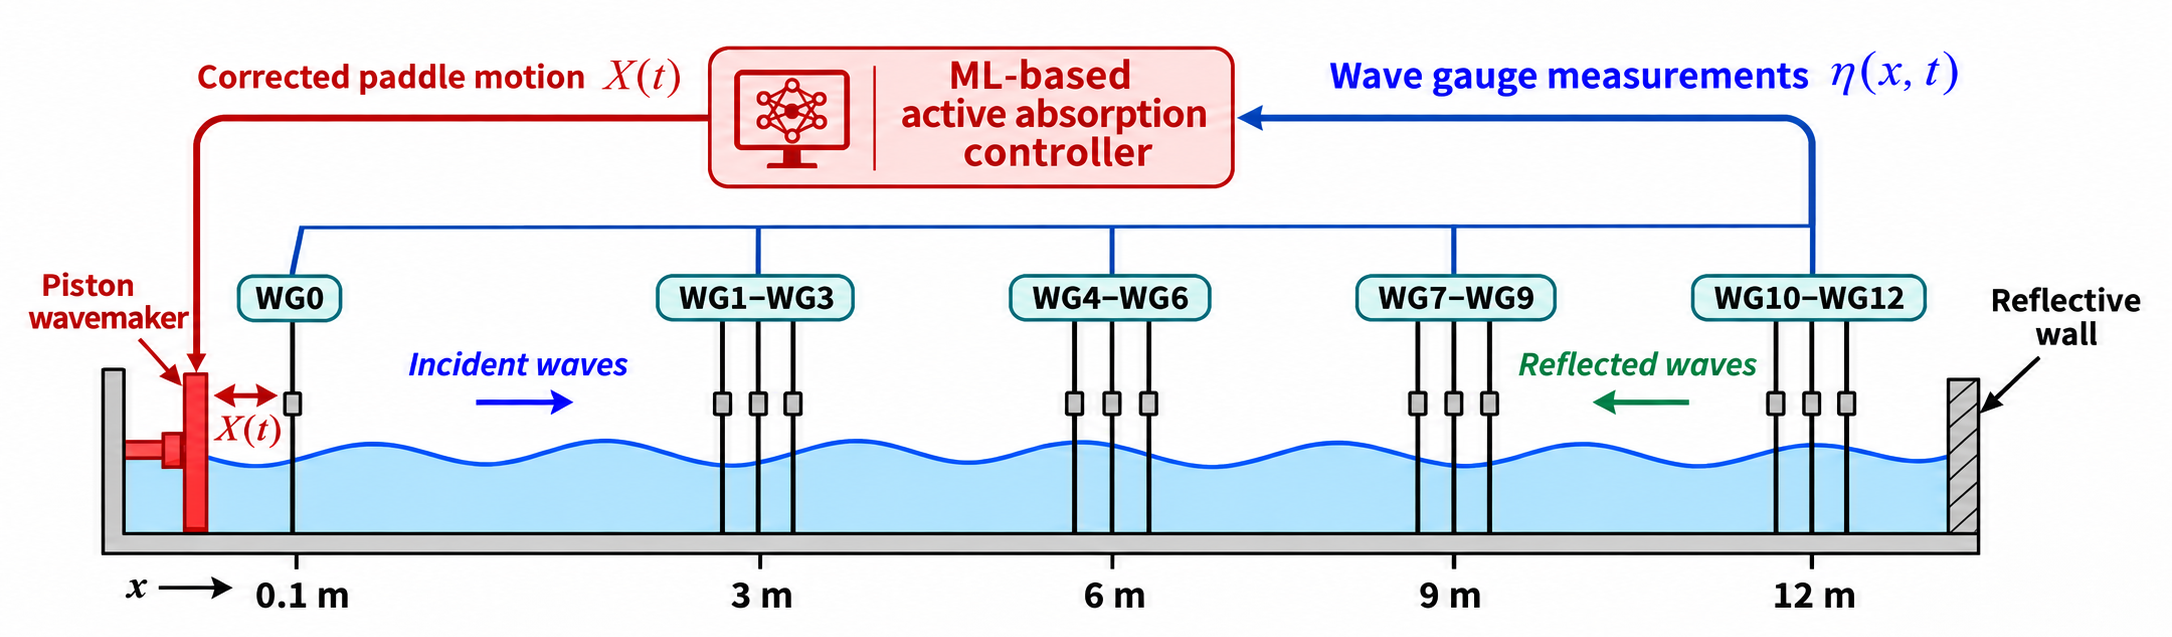
\includegraphics[width=\linewidth]{ml_controlled_wave_flume_schematic_2.png}


% ---- Closed-loop control flow (planned method, not presented as result) ----
{\bfseries\color{metured}\fontsize{10.5}{12}\selectfont Research workflow}\hfill
{\color{muted}\fontsize{8}{9}\selectfont planned ML-controlled stage indicated}\par
\vspace{1.0mm}
\noindent\resizebox{\linewidth}{!}{%
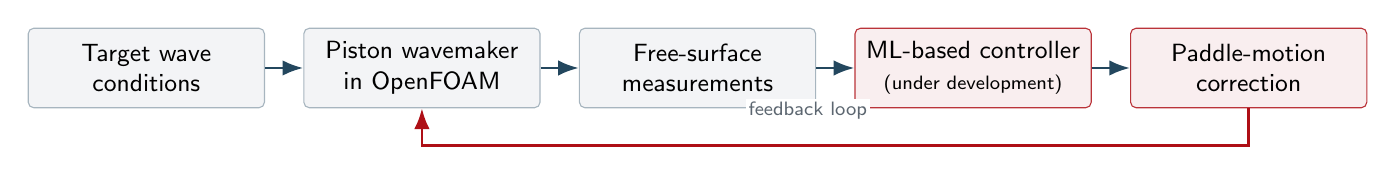
\begin{tikzpicture}[>=Latex,font=\sffamily]
  \tikzset{flowbox/.style={draw=navy!40,fill=cloud,rounded corners=2.0pt,
      align=center,minimum width=3.0cm,minimum height=1.01cm,
      font=\small,inner sep=3pt},
      mlflowbox/.style={draw=metured!85,fill=metured!7,rounded corners=2.0pt,
      align=center,minimum width=3.0cm,minimum height=1.01cm,
      font=\small,inner sep=3pt}}
  \node[flowbox] (a) at (1.6,0) {Target wave\\conditions};
  \node[flowbox] (b) at (5.1,0) {Piston wavemaker\\in OpenFOAM};
  \node[flowbox] (c) at (8.6,0) {Free-surface\\measurements};
  \node[mlflowbox] (d) at (12.1,0) {ML-based controller\\\scriptsize (under development)};
  \node[mlflowbox] (e) at (15.6,0) {Paddle-motion\\correction};
  \foreach \from/\to in {a/b,b/c,c/d,d/e}{\draw[->,line width=1pt,navy] (\from)--(\to);}
  \draw[->,line width=1pt,metured] (e.south)--++(0,-0.47)-|(b.south);
  \node[font=\scriptsize,muted,fill=white,inner sep=1pt] at (10.0,-0.54) {feedback loop};
\end{tikzpicture}}

\SectionHeading{Seminar Focus}
{\fontsize{9.55}{12.3}\selectfont
\FocusItem{Problem:}{Reflections and repeated re-reflections in laboratory wave flumes distort the intended wave field and limit the accuracy of physical model tests.}
\FocusItem{Numerical framework:}{An OpenFOAM numerical flume with a moving piston-type wavemaker is used to study wave generation and free-surface response.}
\FocusItem{Research approach:}{Numerical wave-gauge signals and wavemaker motion are investigated to support a data-driven, real-time active-absorption controller.}
\FocusItem{Evaluation:}{The intended assessment compares different absorption configurations using surface-elevation records and wave-reflection estimates.}
}

\SectionHeading{About the Speaker}
{\fontsize{9.3}{11.6}\selectfont
\SpeakerName\ holds a B.S. in Civil Engineering from Middle East Technical University and is pursuing an M.S. in Coastal and Harbor Engineering at METU. The ongoing thesis focuses on OpenFOAM-based numerical modelling of wave flumes and the development of machine-learning-assisted active wave absorption for piston-type wavemakers.\par
}
\SectionHeading{When \& Contact}
\vspace{-6mm}
\begin{tcolorbox}[enhanced,colback=white,colframe=metured,boxrule=0.75pt,
  arc=1.5mm,left=3mm,right=3mm,top=2mm,bottom=2mm]
\fontsize{9.1}{11}\selectfont
\begin{tabularx}{\linewidth}{@{}>{\bfseries}p{12mm}X@{\hspace{3mm}}>{\bfseries}p{10mm}X@{}}
Date & \SeminarDate \hspace{3cm}& Time & \SeminarTime\\[1mm]
Place & \SeminarRoom & Email & \SpeakerEmail
\end{tabularx}
\end{tcolorbox}
\vspace{1.2mm}
{\color{muted}\rule{\linewidth}{0.45pt}}\vspace{0.8mm}
{\fontsize{8}{9}\selectfont\bfseries CE520 Graduate Seminar -- Fall 2026\hfill Middle East Technical University}
\end{document}
